
\documentclass[12pt]{report}
\usepackage{aums}       % For Master's papers
% \usepackage{auphd}     % For Ph.D.
%\usepackage{auhonors}  % For honors college
\usepackage{ulem}       % underlining on style-page; see \normalem below
\usepackage{url}
\usepackage{tikz}
\usepackage{pgf}
\usepackage[intoc]{nomencl}
\usepackage{graphicx}
\usepackage{hyperref}
\graphicspath{ {./images/} }
\renewcommand{\nomname}{List of Abbreviations}   	       
\makenomenclature 

%% don't forget to run:   makeindex ausample.nlo -s nomencl.ist -o ausample.nls
%% Also, if 
% May want theorems numbered by chapter
% \newtheorem{theorem}{Theorem}[chapter]

% Put the title, author, and date in. 
\title{Sleep Stage Prediction via Deep Learning
using Actigraphy Data to Detect Disorders
by Modeling Sleep}
\author{Omar Barazanji} 
\date{May 10, 2022} %date of graduation
\copyrightyear{2022} %copyright year

\keywords{Deep Learning, Time-Series Forecasting, Health, Sleep}

% Put the Thesis Adviser here. 
\adviser{Dr. SueAnne Griffith}

% Put the committee here (including the adviser), one \professor for each. 
% The advisor must be first, and the dean of the graduate school must be last.
% \professor{Thaddeus Roppel, Chair, Associate Professor of Electrical and Computer Engineering}

% \professor{Prathima Agrawal, Ginn Distinguished Professor of Electrical and Computer Engineering}

\professor{SueAnne Griffith, Professor of Electrical and Computer Engineering}

\begin{document}

\begin{romanpages}      % roman-numbered pages 

\TitlePage 

% \begin{abstract} 
%   In this study, we use datasets \cite{zhang}\cite{bessone} on regular sleep activity to train a model that can accurately predict and label sleep/wake from actigraphy. We created a
%   custom dataset on patients with known disorders that affect sleep, through a mix of
%   public datasets and sleep studies, to add labels for each person’s known disorder.
%   With the disorder labels on the actigraphy data, our trained model will be able to
%   predict if a person is healthy or shows behaviors similar to a known disorder.
% \end{abstract}

\begin{abstract} 
  Sleep scoring is a critical task in sleep medicine that involves the labeling of a patent's sensor data from electroencephalography (EEG), electrocardiography (ECG), and electrooculography (EOG) into different 5 different sleep stages. In this study, we compare the performance of three deep learning models for sleep scoring using actigraphy data and sleep study data. Actigraphy data was used solely for sleep/wake prediction, while sleep lab data (EEG, ECG, and EOG) was used for sleep scoring. This study aims to compare the accuracy of these models, with a focus on identifying the optimal model for each task. For actipgraphy sleep/wake predcition, the dataset consisted of a total of 109 subjects, and each subject's data was divided into training and testing sets. For the sleep lab dataset, the dataset consisted of 30 subjects each with 5 nights of sleep data. The results show that the CNN-LSTM model achieved the highest accuracy for sleep staging. The XGBoost and LSTM models achieved accuracies of 82.3\% and 79.6\%, respectively. These findings suggest that the CNN-LSTM model may be a promising approach for sleep staging using actigraphy data and sleep lab data.
\end{abstract}


\begin{acknowledgments}
  The National Sleep Research Resource was supported by the U.S. National Institutes of Health, National Heart Lung and Blood Institute (R24 HL114473, 75N92019R002).
\end{acknowledgments}

\tableofcontents
\listoffigures
% \listoftables

\printnomenclature[0.5in] %used for the List of Abbreviations
\end{romanpages}        % All done with roman-numbered pages


\normalem       % Make italics the default for \em


\chapter{Introduction}

Sleep is a fundamental biological process that is critical for maintaining overall health and wellbeing. Sleep disorders, such as sleep apnea and insomnia, can have significant negative impacts on an individual's quality of life and can lead to a range of adverse health outcomes. Sleep scoring, the process of identifying and labeling the different stages of sleep, is an essential tool in the diagnosis and treatment of sleep disorders.

Traditionally, sleep scoring has been done manually by trained clinicians. However, the process is time-consuming and subject to inter-rater variability, which can lead to inaccuracies. Recent advances in deep learning models have shown promise in automating the sleep scoring process, making it faster and more accurate.

In this study, we aim to compare the performance of three deep learning models for sleep scoring using both actigraphy data and sleep study data. Actigraphy data is a non-invasive method of measuring activity levels that is often used to track sleep/wake cycles. Our study will use actigraphy data solely for sleep/wake prediction, while sleep study data (EEG, ECG, and EOG) will be used for sleep scoring.

The study aims to identify the optimal model for each task and compare their accuracies. We will evaluate the performance of the CNN-LSTM, XGBoost, and LSTM models on a dataset of 50 subjects, with each subject's data divided into training and testing sets. Our results will provide insights into the potential of deep learning models for sleep scoring using both actigraphy and sleep study data. 

\section{Objective}

In this study, we used datasets on regular sleep activity to train a model that can accurately predict and label sleep/wake from actigraphy. We then will create a custom dataset on patients with known disorders that affect sleep. Through a mix of public datasets and sleep studies, we can add labels for each person's known disorder. With the disorder labels on the actigraphy data, our trained model will be able to predict if a person might have certain disorders or not, such as Insomnia.

\pagebreak

\section{Datasets}

We used various datasets in this study and will be referenced throughout the paper. The first dataset is Sleep Actigraphy from the Urban Poor in India, and it contains 3-axis accelerometer data from 30 participants. Data is labeled with sleep status, either a 1 or a 0 for asleep or awake, respectively. The other dataset comes from Sleep as Android Watch Actigraphy. This dataset contains labels for sleep stages as well as lux (light in lumens), snoring, bpm, and more. Data is collected from a compatible Wear OS device during sleep and is converted into a single actigraphy curve for sleep stage prediction.

\subsection{Sleep Actigraphy from the Urban Poor in India}
Need to add...

\subsection{Sleep as Android Watch Actigraphy}
Need to add...

\pagebreak

\begin{figure}
  \begin{center}
    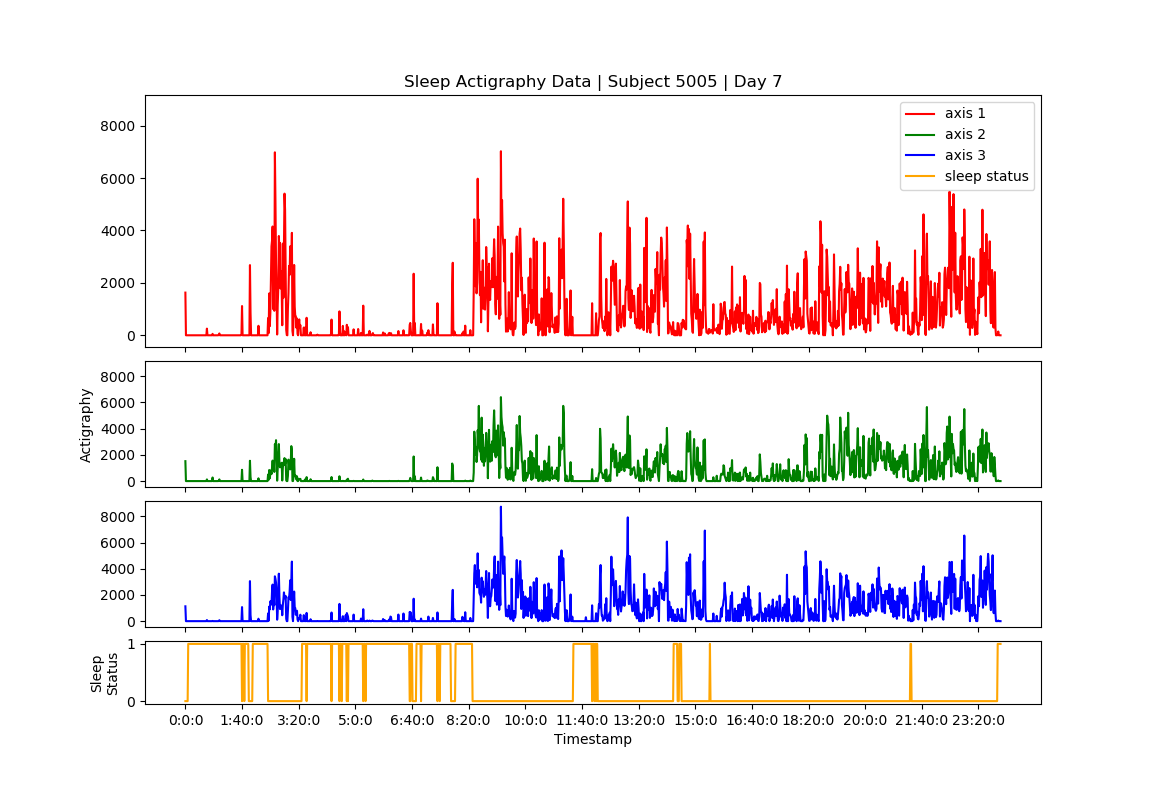
\includegraphics[width=1\linewidth]{model_test_subject5005_day7}
    \caption{Sleep Actigraphy from the Urban Poor in India\cite{zhang}\cite{bessone}}
    \label{urban-poor}
  \end{center}
\end{figure}

\begin{figure}
  \begin{center}
    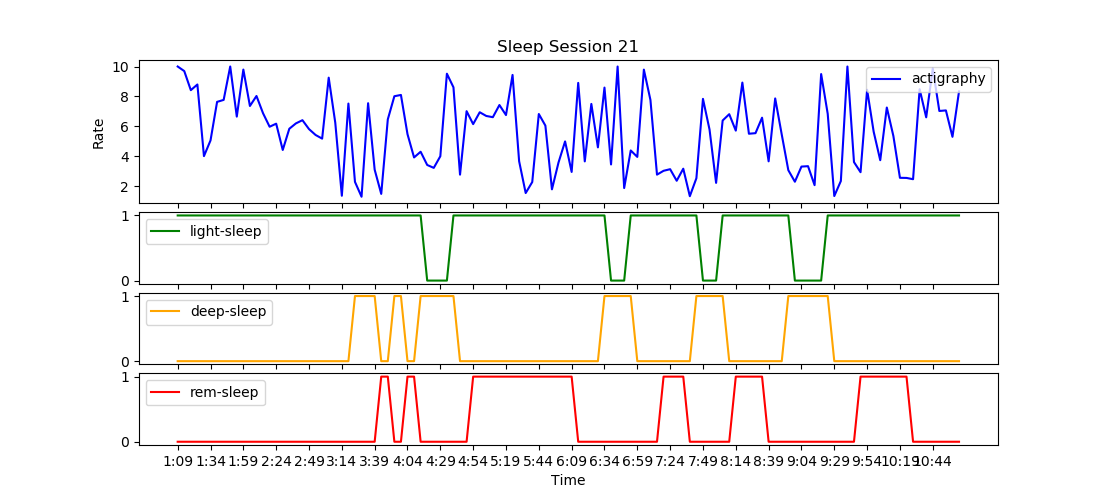
\includegraphics[width=1\linewidth]{REM_NREM_labels}
    \caption{Sleep as Android Watch Actigraphy}
    \label{sleep-android}
  \end{center}
\end{figure}

\chapter{Methods}

We present various methods for sleep/wake prediction, sleep stage prediction, and disorder prediction. We explore popular known methods using XGBoost, SVM, and RNN model architectures. In this paper we propose a new method for sleep-stage classification and sleep/wake classification. Our baseline method will be the vanilla LSTM and we will compare this against our newly proposed methods using the Transformer architecture and another model using a Bidirectional LSTM. 

\section{Sleep/Wake Prediction}
Recurrent Neural Networks (RNNs) are a special type of neural network that are designed to process long sequences of data and predict how a series of data should continue per time step. The Long Short-Term Memory (LSTM) network is a refined version of the vanilla RNN that can "forget" useless information in training data. This prevents the network from overfitting, which is a big problem in the vanilla RNN. Looking at sleep actigraphy data as a time series problem makes the prediction of any label from the training data quite simple. For example, figure \ref{urban-poor} above shows the x, y, and z activity data from the accelerometers on a participant's wrist, and the sleep status (1=asleep, 0=awake) shows when the person is asleep or awake in time with the accelerometer. We can sub-sample all 4 labels together with a window size of T, usually around T=30, and predict sleep status or anyother variable that was recorded along with the accelerometer per time step. 

\begin{figure}
  \begin{center}
    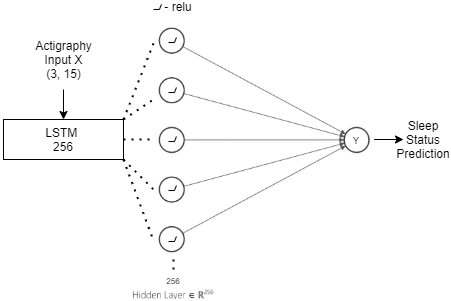
\includegraphics[width=0.7\linewidth]{sleep_status_LSTM_model}
    \caption{LSTM Model with 256 units for Sleep/Wake Prediction}
    \label{lstm-architecture}
  \end{center}
\end{figure}

\section{Sleep Stage Prediction}
To classify sleep stages as multiple labels during sleep from actigraphy data, we will need to use a multi-variate LSTM that can output more than one label per time step. To do this we will update our vanilla LSTM model's output Y from figure \ref{lstm-architecture} to have a dimension equal to the number of desired sleep stage labels. For our dataset shown in \ref{sleep-android}, we can predict light, deep, and REM sleep stages. We can also add sleep/wake from the Sleep as Android dataset to have a total of 4 output labels per timestep. 

\section{Disorder Prediction}
Need to add...

\chapter{Results}

Results for sleep/wake predcition using the LSTM network with 256 units can be seen below in figures \ref{lstm-loss} and \ref{lstm-accuracy}. The model performs at 92 percent accuracy with 256 units and 15 training epochs. 

\section{Sleep/Wake Results}
Need to add...

\subsection{XGBoost}
Need to add...

\subsection{SVM}
Need to add...

\subsection{LSTM}
Need to add...

\subsection{Transformer}
Need to add...

\section{Sleep Stage Results}
Need to add...

\subsection{XGBoost}
Need to add...

\subsection{SVM}
Need to add...

\subsection{LSTM}
Need to add...

\subsection{Transformer}
Need to add...

\begin{figure}
  \begin{center}
    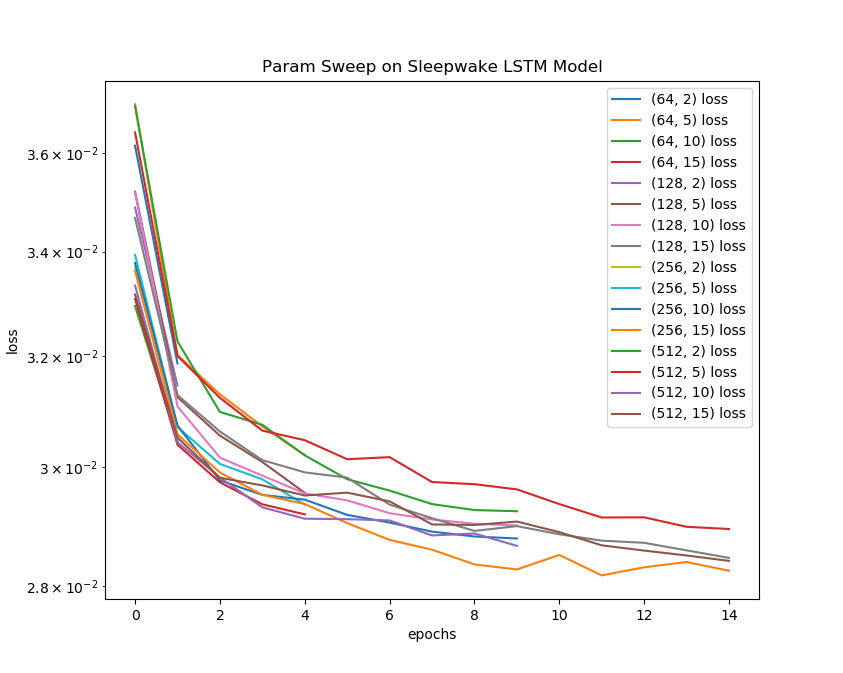
\includegraphics[width=0.9\linewidth]{param_sweep_loss}
    \caption{Loss on Model with 256 units for Sleep/Wake Prediction during Training}
    \label{lstm-loss}
  \end{center}
\end{figure}

\begin{figure}
  \begin{center}
    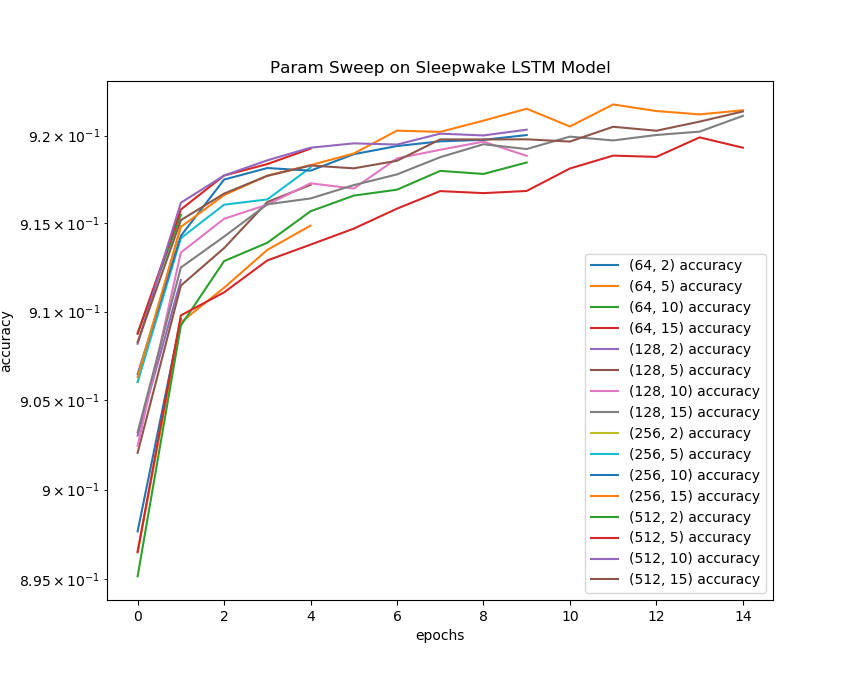
\includegraphics[width=0.9\linewidth]{param_sweep_accuracy}
    \caption{Accuracy on Model with 256 units for Sleep/Wake Prediction during Training}
    \label{lstm-accuracy}
  \end{center}
\end{figure}

\chapter{Conclusion}
Need to add...

\section{Discussion}
Need to add...

\section{Conclusion}
Need to add...

\begin{thebibliography}{99}
\newcommand{\AmS}{$${\protect\the\textfont2 A}\kern-.1667em\lower
         .5ex\hbox{\protect\the\textfont2 M}\kern
         -.125em{\protect\the\textfont2 S}}

\bibitem{iber} C. Iber, S. Ancoli-Israel, A. L. Chesson, and S. F. Quan, The AASM manual for the scoring of sleep and associated events : rules, terminology, and technical specifications. Istchester, IL: American Academy of Sleep Medicine, 2007.

\bibitem{guillot} Guillot, A., Sauvet, F., During, E., Thorey, V. Dreem Open Datasets: Multi-Scored Sleep Datasets to compare Human and Automated sleep staging, 2019.

\bibitem{cho} Cho, J.H.; Choi, J.H.; Moon, J.E.; Lee, Y.J.; Lee, H.D.; Ha, T.K. Validation Study on Automated Sleep Stage Scoring Using a Deep Learning Algorithm. Medicina 2022, 58, 779.

\bibitem{zhang} Zhang GQ, Cui L, Mueller R, Tao S, Kim M, Rueschman M, Mariani S, Mobley D, Redline S. The National Sleep Research Resource: towards a sleep data commons. J Am Med Inform Assoc. 2018 Oct 1;25(10):1351-1358. doi: 10.1093/jamia/ocy064. PMID: 29860441; PMCID: PMC6188513.

\bibitem{bessone} Bessone P, Rao G, Schilbach F, Schofield H, Toma M. The Economic Consequences of Increasing Sleep Among the Urban Poor. Q J Econ. 2021 Apr 8;136(3):1887-1941. doi: 10.1093/qje/qjab013. PMID: 34220361; PMCID: PMC8242594.

\bibitem{sano} A. Sano, W. Chen, D. Lopez-Martinez, S. Taylor and R. W. Picard, "Multimodal Ambulatory Sleep Detection Using LSTM Recurrent Neural Networks," in IEEE Journal of Biomedical and Health Informatics, vol. 23, no. 4, pp. 1607-1617, July 2019, doi:10.1109/JBHI.2018.2867619.

\bibitem{sathyanarayana} Sathyanarayana, Aartietal. “Sleep Quality Prediction From Wearable Data Using Deep Learning.” JMIR mHealth and uHealth vol. 4, 4e125.4Nov.2016, doi:10.2196/mhealth.6562.

\bibitem{chen} Chen, Tianqi, Carlos Guestrin. 'XGBoost'. Proceedings of the 22nd ACM SIGKDD International Conference on Knowledge Discovery and Data Mining. ACM, 2016. Web.

\bibitem{shantilal} Shantilal, K. D. Donohue and B. F. O'Hara, "SVM for automatic rodent sleep-wake classification," IEEE SoutheastCon 2008, 2008, pp. 581-586, doi: 10.1109/SECON.2008.4494360.

\bibitem{vaswani} Vaswani, Ashish, Noam Shazeer, Niki Parmar, Jakob Uszkoreit, Llion Jones, Aidan N. Gomez, Lukasz Kaiser, Illia Polosukhin. 'Attention Is All You Need'. arXiv, 2017. 

\end{thebibliography}



\appendix
\chapter*{Appendices\addcontentsline{toc}{chapter}{Appendices}}

\chapter{Source Code}

\begin{singlespace}
Code link
\end{singlespace}

\end{document}